\subsection{Merkle 快照与完整性验证实现}

Merkle 快照与完整性验证是 FoodShield 可信审计能力的核心。系统在消息写入数据库后，会根据当前订单内所有消息哈希构建 Merkle Tree，并生成 Merkle Root 快照。该 Root 代表某一时刻该订单通信记录的完整性状态。

在快照生成过程中，系统首先按照消息写入顺序读取目标订单的 \texttt{message\_hash} 列表，将每条消息哈希作为 Merkle Tree 的叶子节点。然后，系统对相邻叶子节点进行拼接并计算 SM3 哈希，逐层向上构建父节点，最终得到唯一的 Merkle Root。若某一层节点数为奇数，则复制最后一个节点参与下一层计算。计算完成后，系统将订单号、消息数量、Root 值、快照时间和操作类型写入 \texttt{audit\_logs} 表。

\begin{figure}[H]
    \centering
    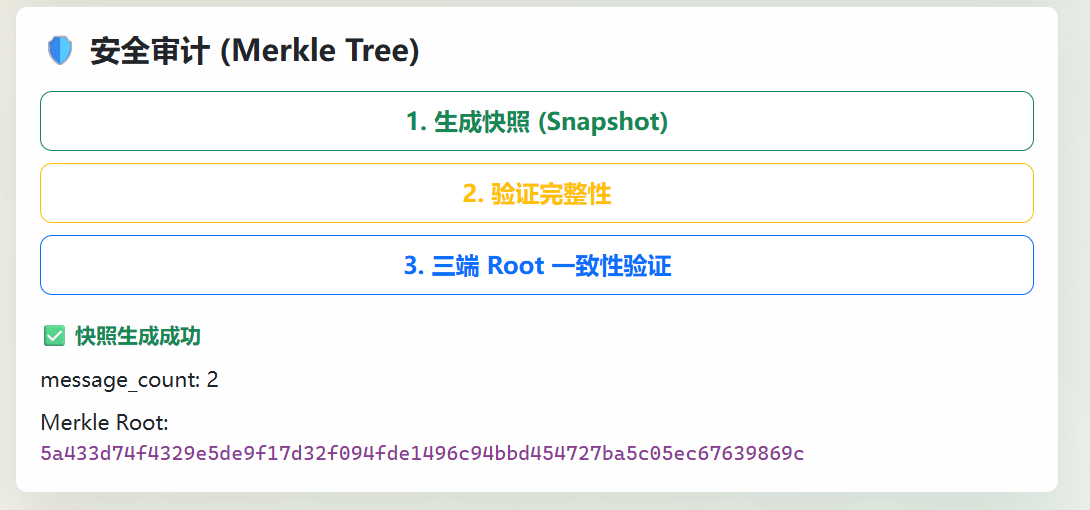
\includegraphics[width=0.95\textwidth]{content/chapter4/merkle_snapshot_result.png}
    \caption{Merkle Root 快照生成结果}
    \label{fig:merkle-snapshot-result}
\end{figure}

完整性验证时，管理员端提交目标订单号，服务器重新读取该订单当前消息记录，并重新计算每条消息的哈希值。随后，系统以重新计算得到的哈希序列构建新的 Merkle Root，并与 \texttt{audit\_logs} 表中保存的历史快照 Root 进行比对。若两者一致，说明当前通信记录与快照生成时保持一致；若两者不一致，则说明消息内容、消息数量或消息顺序可能被修改。

系统能够检测以下几类篡改行为：

\begin{enumerate}
    \item 修改消息内容：重新计算的消息哈希发生变化，导致 Root 不一致；
    \item 删除历史消息：叶子节点数量变化，导致 Root 不一致；
    \item 插入伪造消息：新增叶子节点，导致 Root 不一致；
    \item 重排消息顺序：叶子节点顺序变化，导致 Root 不一致；
    \item 修改消息元数据：时间戳、角色或订单号变化，导致消息哈希变化。
\end{enumerate}

完整性验证流程可以抽象为：
\begin{figure}[H]
    \centering
    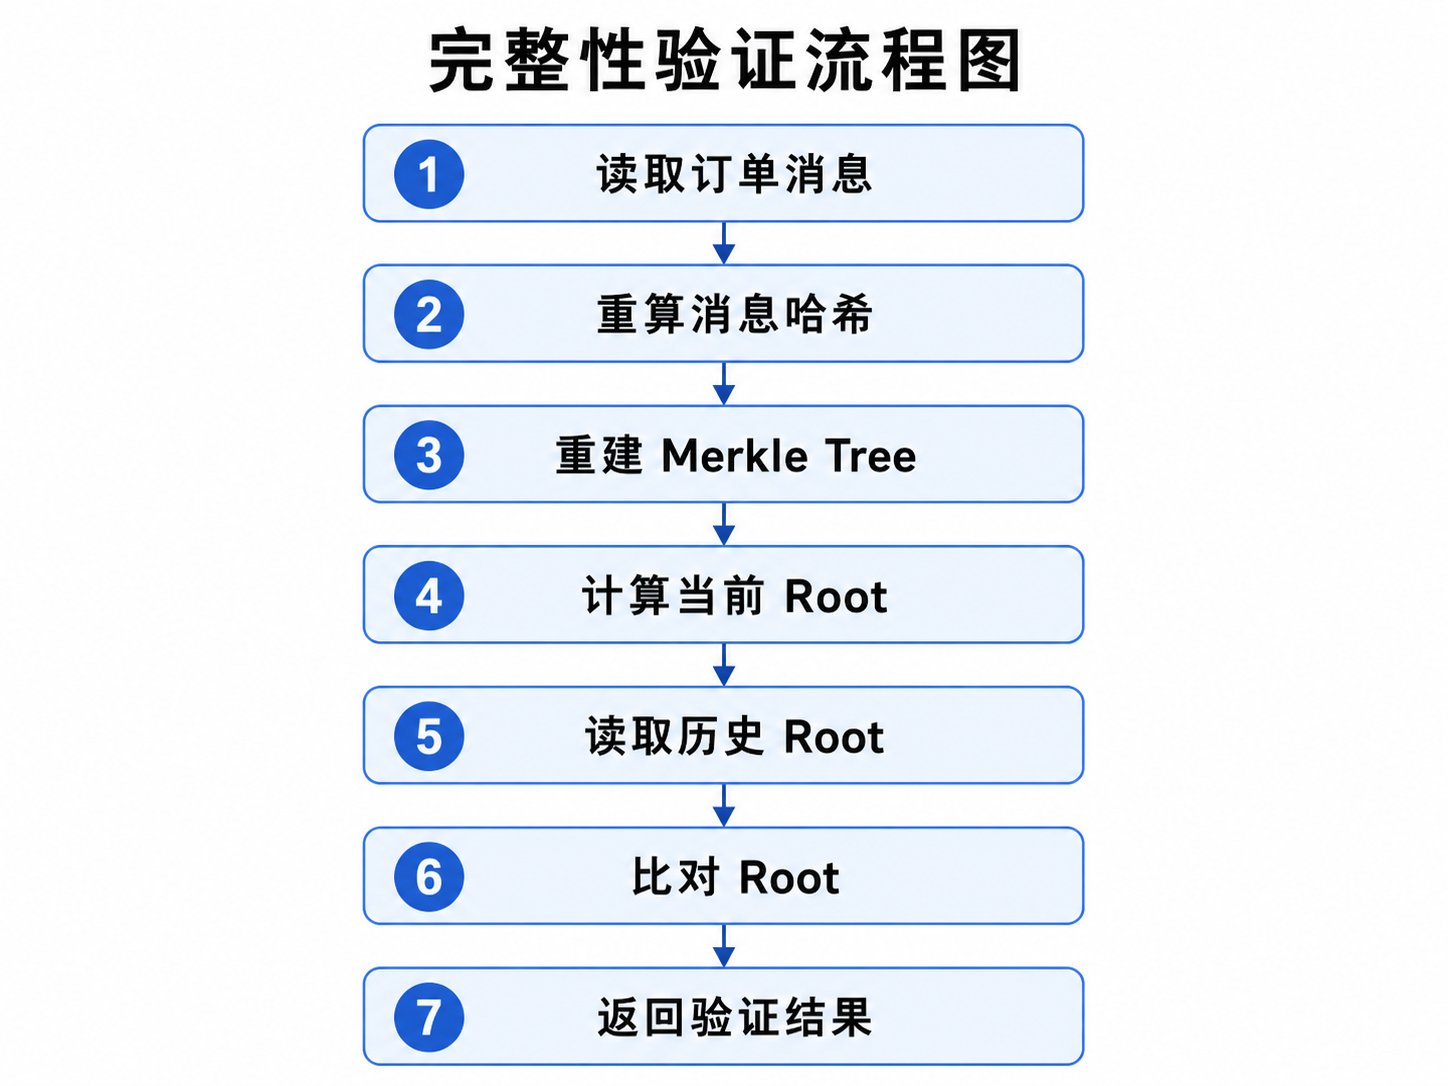
\includegraphics[width=0.82\textwidth]{content/chapter4/verify_flow.png}
    \caption{完整性验证流程图}
    \label{fig:verify-flow}
\end{figure}

\begin{figure}[H]
    \centering
    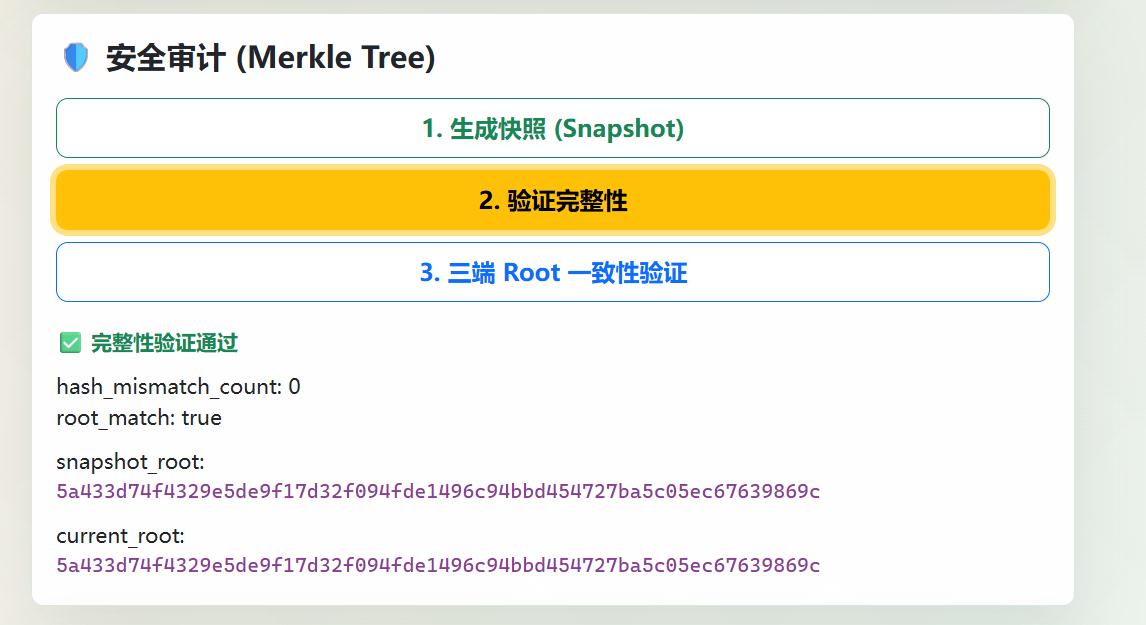
\includegraphics[width=0.95\textwidth]{content/chapter4/verify_ok.png}
    \caption{日志完整性验证通过结果}
    \label{fig:verify-ok}
\end{figure}

此外，系统实现了三端摘要一致性增强机制。服务器在消息更新后将最新 Merkle Root 推送给用户端和骑手端，客户端可将 Root 保存在本地，并在审计时主动上报。管理员验证时可以将服务端快照 Root、用户端上报 Root 和骑手端上报 Root 进行三方比对。若三者一致，则说明三端对订单通信摘要状态达成一致；若不一致，则提示可能存在日志篡改、客户端异常或上报数据不一致。

\begin{figure}[H]
    \centering
    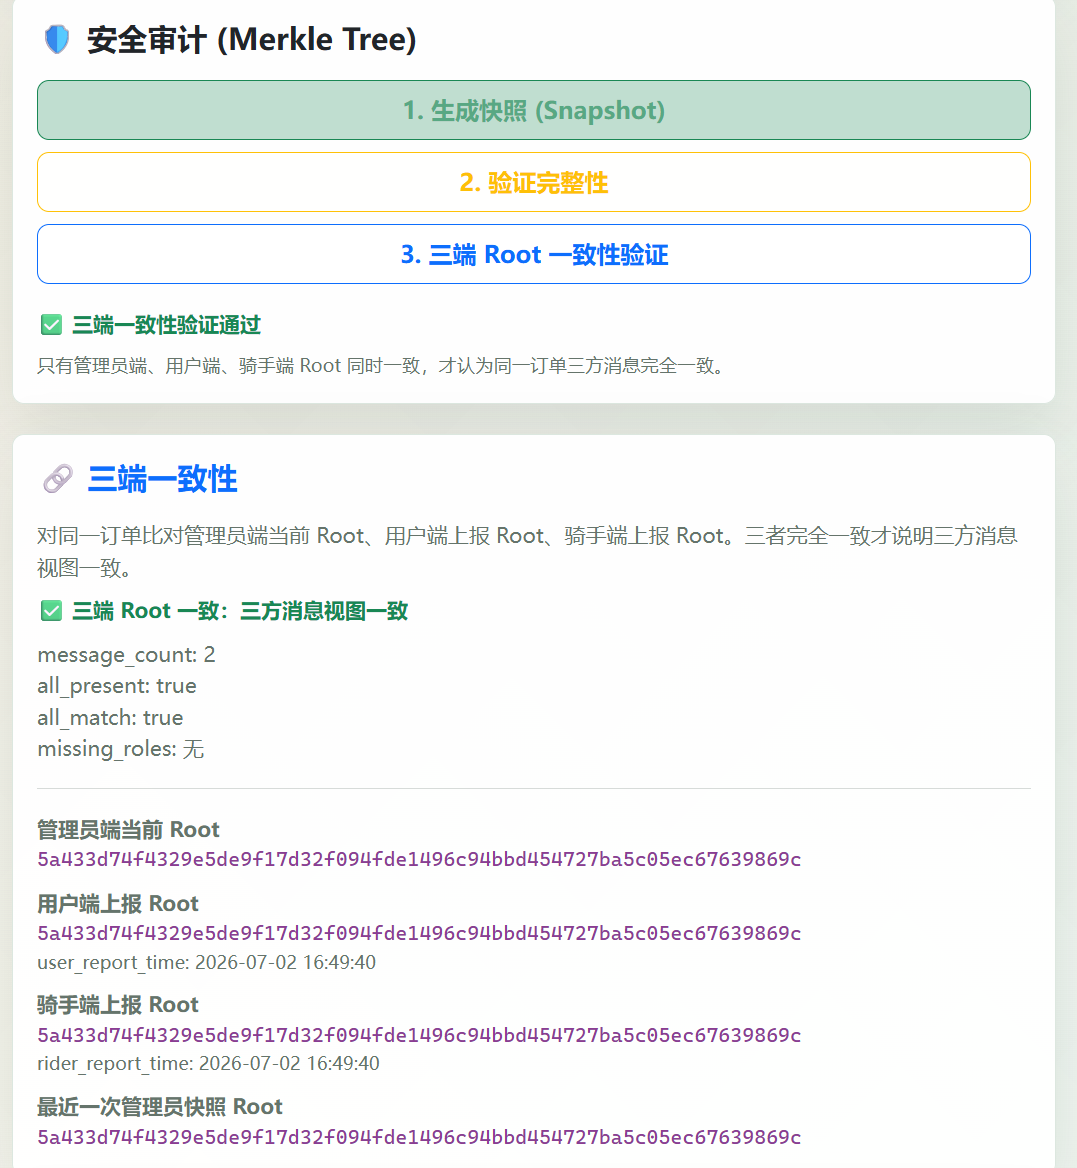
\includegraphics[width=0.95\textwidth]{content/chapter4/three_party_root.png}
    \caption{三端摘要一致性验证结果}
    \label{fig:three-party-root}
\end{figure}
